\chapter{Методы и материалы}
\section{NS-2}
NS-2(Network simaulator 2) — это программное средство моделирования сетей, использующиеся 
для исследования и анализа поведения компьютерных сетей. 
Запуск симуляции в данной среде позволяет анализировать различные протоколы и алгоритмы сетевой связи. 
NS-2 разработан на языке программирования С++ и TCL, что обеспечивает гибкость и расширяемость средства моделирования. 
NS-2 содержит библиотеку классов, представляют различные элементы сети, такие как узлы, маршрутизаторы, каналы связи и протоколы передачы данных. Для создания модели сети определяются характеристики и параметры каждого элемента сети: пропускная способность каналов, задержки, вероятность потери пакетов и другие. После завершения симуляции NS-2 предоставляет мощные инструменты анализа результатов, включая возможность визуализации данных посредством программы NAM(Network animator), статический анализ и сравнение экспериментов, что позволяет изучать и оценивать производительность различных протоколов и алгоритмов в различных сценариях сети~\cite{The2011,Floyd1997}.

\section{Mininet}
Mininet — это симулятор сетевых топологий на основе виртуаилизации, который позволяет моделировать и изучать поведение сетей в контролируемой среде, основанный на использовании виртуальных машин и пространств имен Linux для создания изолированных сетевых узлов. Моделирование сетевых топологией с помощью Mininet позволяет исследовать различные сетевые протоколые, маршрутизацию, управление трафиком и т. д. Возможности моделирования с помощью Mininet включают создание виртуальных сетевых узлов, конфигурирование топологий(связь между узлами, настраивать IP-адреса, маршрутизацию), имитировать различные условия сети, такие как задержки, потери пакетов и пропускную способность, интеграция с контроллерами для исследования новых протоколов и алгоритмов.

\section{Cisco Packet Tracer}
Packet Tracer — это программное средство, предоставляемое компанией Cisco Systems, позволяющей смоделировать, конфигурировать и отлаживать сетевые сценарии, широко используемое в области сетевых технологий. Данное программное обеспечение предоставляет виртуальную среду, которое позволяет создавать сетевые топологии и настраивать устройства Cisco: маршрутизаторы, коммутаторы, и т д. Графический интерфейс позволяет соединять устройства, устанавливать параметры соединений и задавать настройки протоколов. Cisco Packet Tracer позволяет имитировать передачу данных в сети. Пользователи могут выполнять различные тесты связи, проводить диагностику и мониторинг сетевых устройств, а также создавать и анализировать журналы событий.

\section{GNS-3}
GNS-3 — это программное средство моделирования сетей, позволяющий создавать виртуальные сети, состоящие из реальных или виртуальных устройств, и анализировать их поведение. GNS-3 разработан на языке программирования Python и основан на эмуляторе динамических узлов Dynamips, который позволяет запускать реальные образы операционных систем. В отличие от Packet Tracer, GNS-3 позволяет смоделировать не только устройства Cisco, но и другие устройства, как Juniper, Palo Alto и другие, что позволяет смоделировать различные типы сетей, включая центры обработки данных и облачные инфраструктуры. Одной из главных особенностей GNS-3 является интеграция с виртуальными машинами, что расширяет возможности моделирования. Появляется возможность создавать сетевые сценарии, в которых виртуальные машины выполняют реальные функции, такие как серверы, клиенты, точки доступа Wi-Fi и т. д. Это позволяет проводить натурное моделирование и получить более реалистичные результаты в рамках виртуальной среды.



Эта команда должна работать (см. рис.~\ref{fig:1.1}).


\begin{figure}[!h]
  \centering
  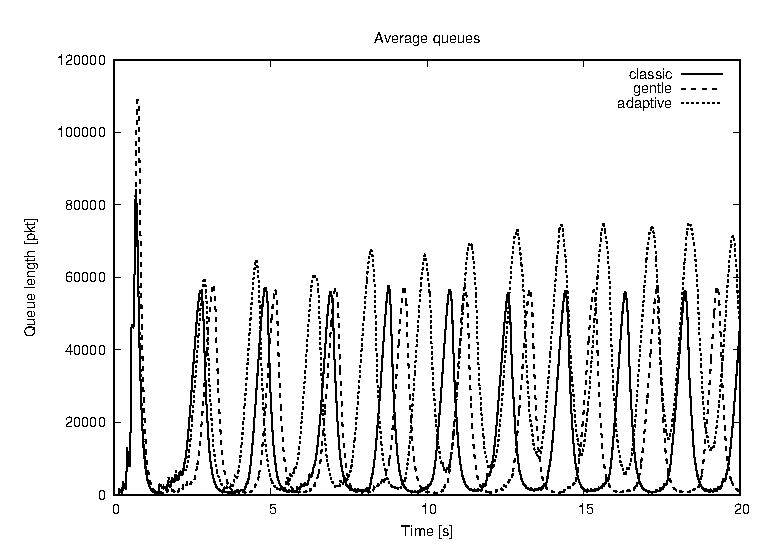
\includegraphics[width=0.9\linewidth]{image/av_queues_3types.eps}
  \caption{3 types of RED}
  \label{fig:1.1}
\end{figure}



\section{SUMO-модель движения транспорта для города Абиджан, коммуны Абобо}


Реализация модели VANET будет сделана для города Абиджан, а точнее для
коммуны Абобо.  Первым шагом будет загрузка xml-файла через карты с
сайта (\url{https://www.openstreetmap.org/.})  Вторым шагом будет
преобразование загруженного файла в xml-формат с помощью команды:
\begin{verbatim}
    netconvert --osm-files filename.osm -o filename.net.xml filename.net.xml
\end{verbatim}

На третьем шаге мы должны использовать файл в нашей папке sumo, мы скопируем
его и поместим в наш проект. Для этого воспользуемся командой:
\begin{verbatim}
    cd /home/directory/sumo-x.x/data/typemap
\end{verbatim}

Последний шаг перед компиляцией будет выполнен с помощью следующей команды
\begin{minted}[linenos,tabsize=2,breaklines]{bash}
    polyconvert --osm-files filename.osm --net-file filename.net.xml, --type-file osmPolyconvert.typ.xml -o filename.poly.xml
    python /home/directory/sumo-x.x/tools/randomtrips.py -n fileName.net.xml -r, fileName.rou.xml -e 50 -l
\end{minted}

Запуск программы (рис.~\ref{fig:1.3}):
\begin{verbatim}
    sumo-gui nomdufichier.sumo.cfg`
\end{verbatim}

\begin{figure}[!h]
  \centering
  \includegraphics[width=0.9\linewidth]{image/08.PNG}
  \caption{Фрагмент SUMO-модели движения транспорта для города Абиджан, коммуны Абобо}
  \label{fig:1.3}
\end{figure}



